\infolevone{
\subsection{SHMS Lead Glass Shower Calorimeter}

The SHMS lead glass shower calorimeter, located behind the S2Y
hodoscope plane, is the last detector in the SHMS detector stack.  It
consists of two sections, a pre-shower layer of 28 TF-1 lead glass 10
cm thick followed by a a fly's eye array of 224 F-101 blocks with a
depth of 50 cm.  (Figure~\ref{fig:shms-shower-1})

\begin{figure}
\begin{center}
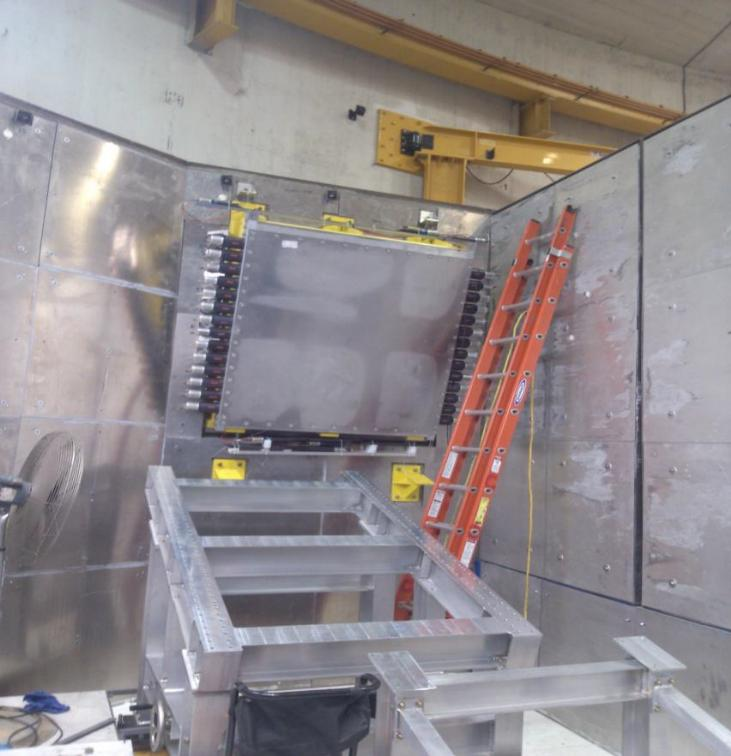
\includegraphics[height=2.5in]{shms-shower-1a.jpg}
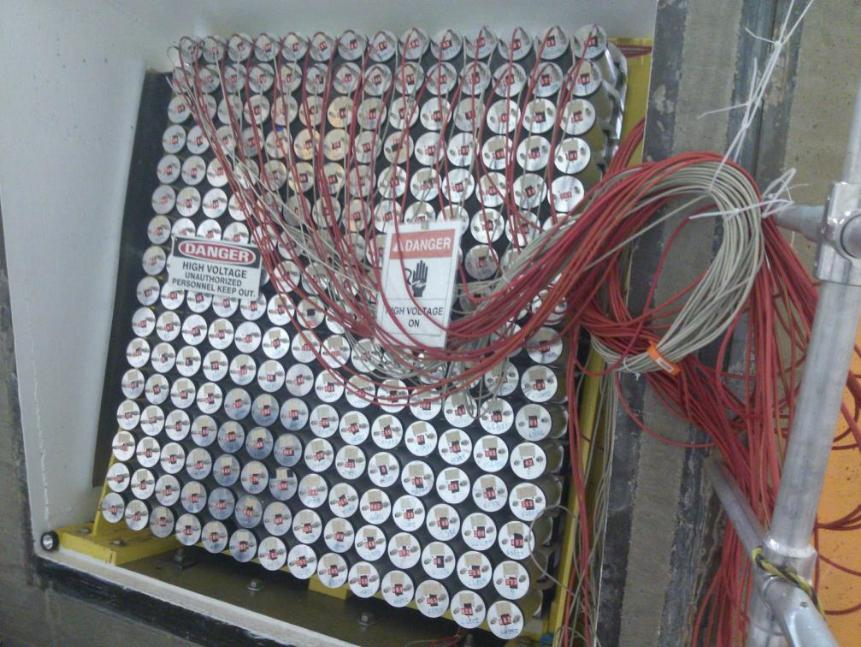
\includegraphics[height=2.5in]{shms-shower-1b.jpg}
\caption{\label{fig:shms-shower-1}Preshower (front view) and Shower
  (back view) parts of the SHMS calorimeter.}
\end{center}
\end{figure}


\subsubsection{Design Overview}

The SHMS lead glass calorimeter is designed for electron/hadron
identification, by means of detection of \v{C}erenkov light from
electromagnetic (EM) showers and hadronic cascades developed in a
dense optical radiator. It consists of 2 parts, dubbed the Shower and
Preshower respectively. The main unit is Shower, which is 18 radiation
lengths deep and ensures total capture of EM showers in the GeV range. The
Preshower is just 3.6 radiation length thick and is positioned before
the Shower. It is to augment PID by detecting the early (relative to
hadronic cascades) onset of EM showers.

TF-1 and F-101 type lead glasses are used as an optical radiator in
the Preshower and Shower respectively (refractive index 1.65, density
3.86 g/cm3). The light output is detected by means of 3 inch Photonis
XP3462B and XP3461 PMTs in the Preshower and Shower respectively (8
stages, flat lime-glass window, bialcali photocathode with peak
quantum efficiency of 29\% at 400 nm).

\begin{figure}
\begin{center}
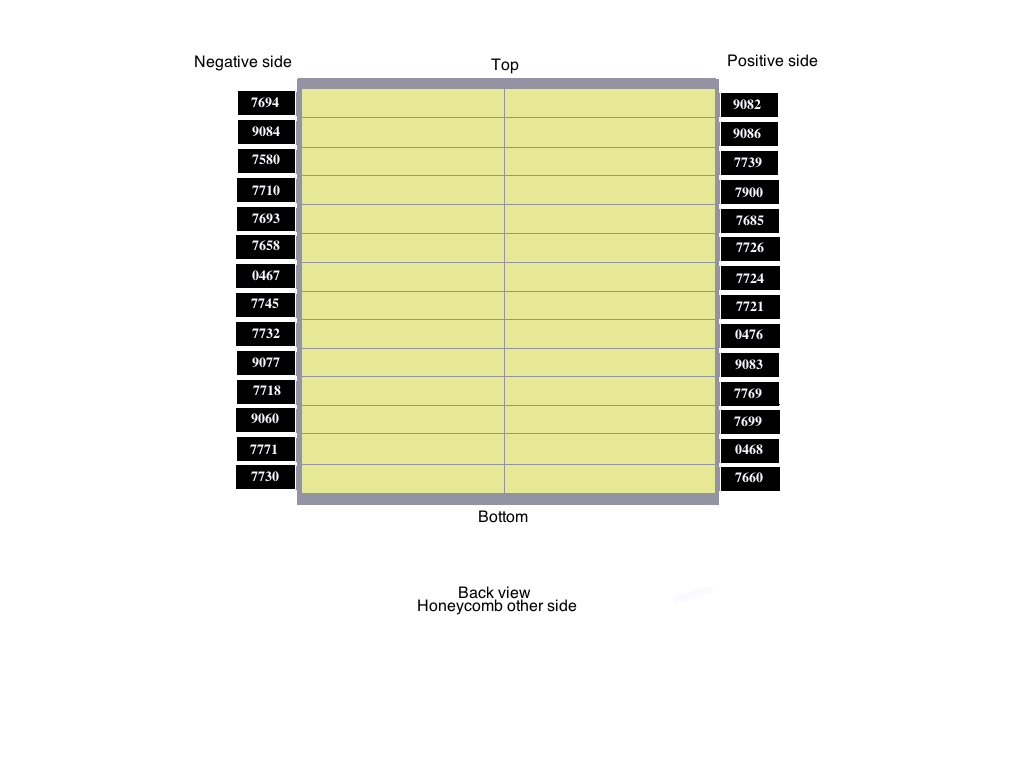
\includegraphics[width=6in,trim={0 5cm 0 1cm}]{shms-shower-3.png}
\caption{\label{fig:shms-shower-3}Schematic of SHMS Preshower as
  viewed from the rear showing PMT serial numbers.}
\end{center}
\end{figure}

The Preshower radiator consists of a layer of 28 TF-1 type $10\times
10\times 70~\textrm{cm}^3$ lead glass blocks from the calorimeter of
the retired SOS spectrometer.
(Figure~\ref{fig:shms-shower-3}  The blocks are stacked in two columns in
an aluminum enclosure. They are optically insulated by a wraping of 50
$\mu$m
thick aluminized Mylar and 10 cm wide strips of 50 $\mu$m thick black
Tedlar film running between them. On both sides of the enclosure
there are 90 mm circular openings, one per block, into which the PMT
cylindrical housings are screwed. Inside the housings, the PMTs are
wrapped in thin Teflon tape and placed in heat shrink tubing for
electric insulation, then are shielded from the fringe fields of the
spectrometer magnets by 6 turns of 10 $\mu$m thick $\mu$-metal foil The PMTs
are optically coupled to the lead glass blocks by means of thin layer
of Bicron ND-703 optical grease (refractive index 1.46). The PMT
sockets protrude from the rear side of the housings, such that PMT
bases are coupled to the sockets outside of the housings.

\begin{figure}
\begin{center}
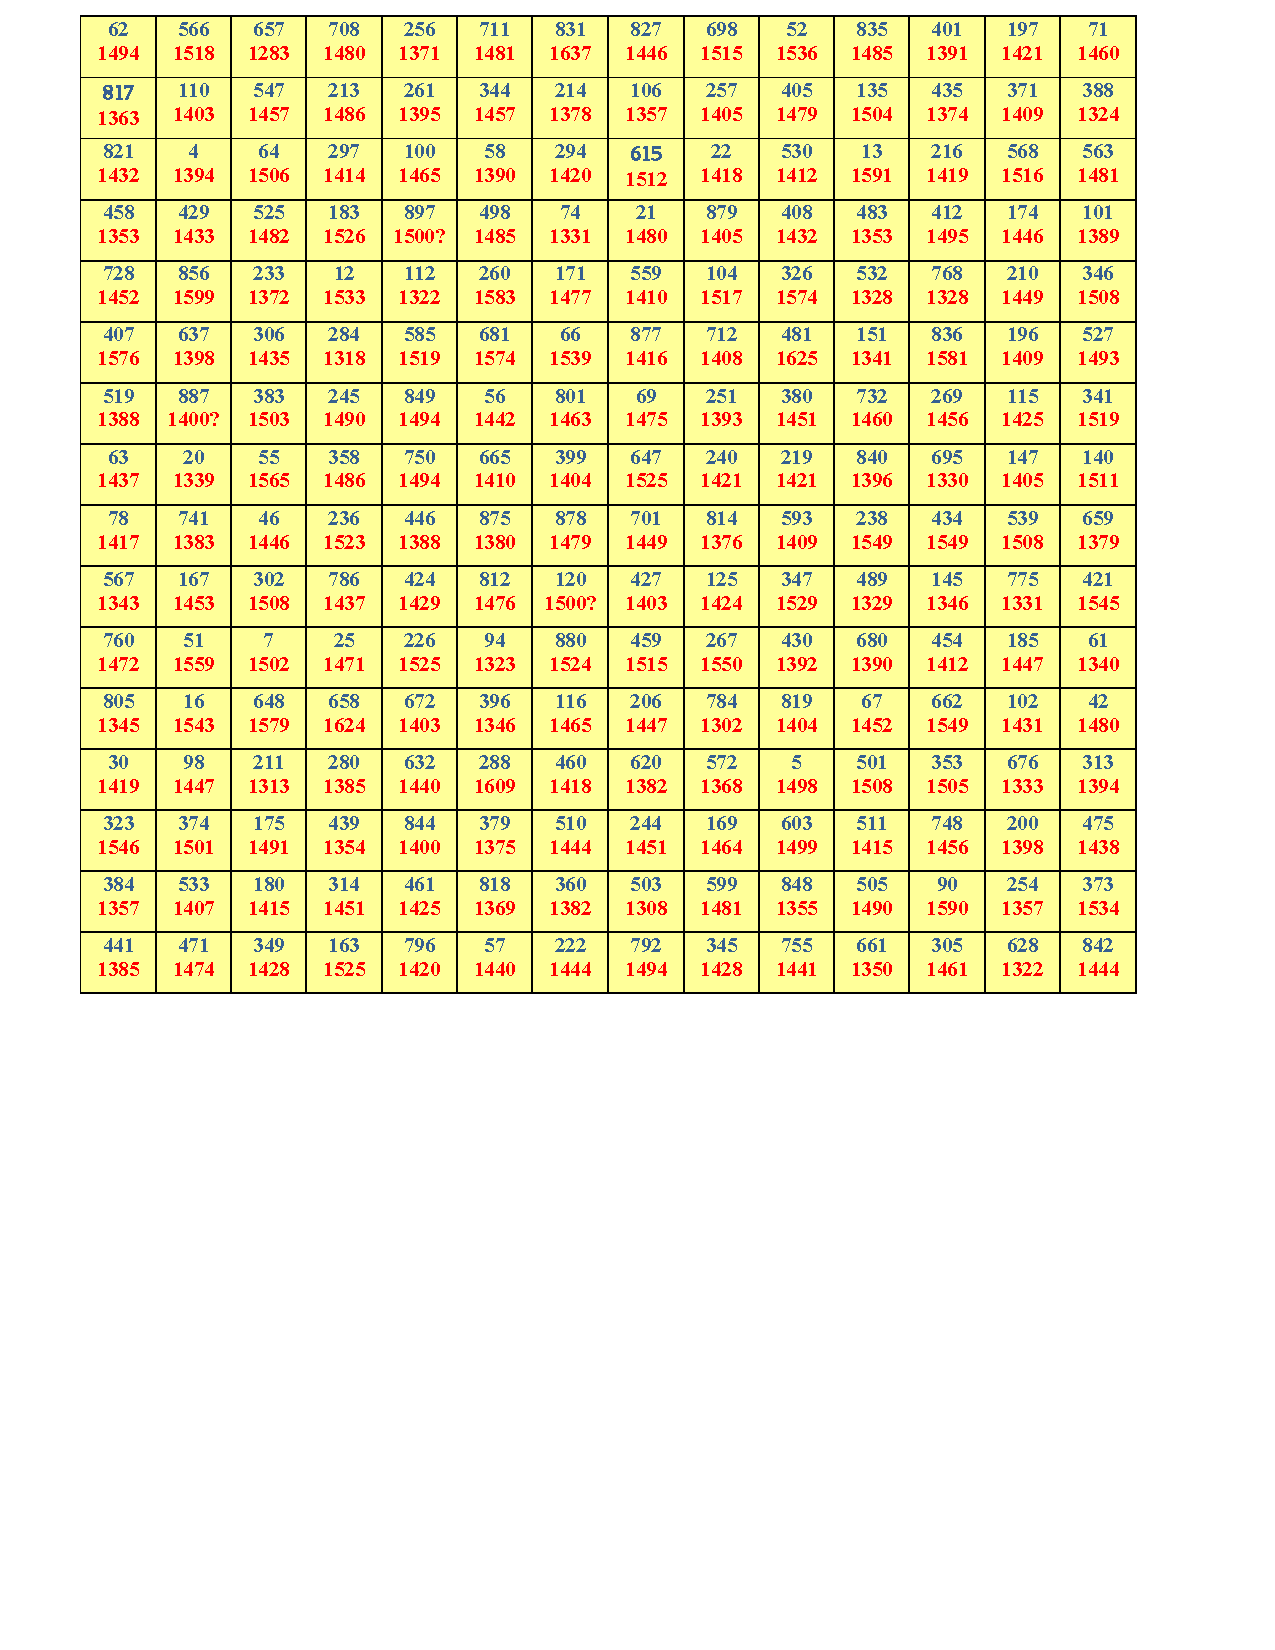
\includegraphics[width=5in,trim={0 10cm 0 0}]{shms-shower-2.pdf}
\caption{\label{fig:shms-shower-2}Schematic of SHMS Shower array as
  viewed from the rear showing block numbers and nonimal high voltages
  taken from the HERMES database.}
\end{center}
\end{figure}

The Shower part consists of 224 modules from the retired HERMES
calorimeter\cite{Avakian199869,AVAKIAN1996155}, stacked in a ``fly’s eye'' configuration of 14 columns
and 16 rows.  (Figure~\ref{fig:shms-shower-2}) Each module is
comprised of a $9\times 9\times 50~\textrm{cm}^3$ F-101 type lead
glass block and a PMT assembly. Each block is wrapped in 50 $\mu$m
aluminize Mylar film and 125 $\mu$m Tedlar paper for optical
insolation. The PMT is surrounded by a 1.5 mm thick $\mu$-metal sheet
and wrapped in 2 layers of Teflon foil for magnetic shielding and
electric insulation correspondingly. The cylindrical aluminum
container of the PMT assembly is fixed to a titanium flange which is
glued to the block. Silgard-184 optical glue with a refractive index
of 1.41 is used for optical coupling of the PMTs to the
blocks. Surface mounted HV divider is pin-to-pin soldered to the PMT.

As a full absorption detector, the calorimeter is positioned at the
very end of the SHMS detector stack. The support stand for the Preshower
is mounted on the back wall of the detector hut. The Shower is
assembled directly behind the Preshower, in a rectangular opening
within the wall. Both sub-detectors are aligned with the central ray of
the spectrometer and are tilted by the SHMS bend angle of $18^{\circ}$ relative
to gravity. Both sides of Preshower are easily accessible from the
detector hut, albeit a ladder is needed to access top PMTs. The back
side of the Shower can be accessed only when SHMS is rotated to $40^{\circ}$ and
aligned with the SHMS service platform.

The drawings of the SHMS calorimeter are available from the Hall C
engineering group.  Expected performance, from simulations, is discussed
in~\cite{Mkrtchyan201385}.





\subsubsection{General Operating Procedures}
The design of the SHMS Preshower permits changing of PMTs and bases during
experimental operations, if needed. In contrast, the construction of the
Shower modules does not assume an easy modification; experts must be
consulted in case of a potential change in the Shower (see list of
responsible personnel below). Spare Shower modules are in Physics
Storage (ask Hall C technicians for assistance).

The photomultiplier tubes and bases are operated at negative high
voltages up to $\unsim 2000~\textrm{V}$. No directly accessible
components carry high voltage. Standard safety precautions for
handling high voltage on photo tubes must be observed, including, but
not limited to disabling the HV at the power supply and disconnecting
the HV cables from the bases (except in limited test cases) whenever
the base covers are removed (to avoid electrical shock), or whenever
optical hermeticity of the detectors is compromised (to avoid damaging
photo-cathodes of the tubes). Personnel shall be careful when
removing a Preshower tube-base assembly, shall avoid mechanical shocks
of the tubes and of the whole assembly in order not to break the glass
tubes and to preserve the properties of the inner $\mu$-metal
shielding.

None of the materials and components used are known to pose any health
or environmental hazards beyond cutting skin from broken glass or
sharp edges.

\subsubsection{Preshower PMT Removal and Replacement}
\subsubsection*{PMT Removal}
\begin{itemize}
\item Make sure all HV’s are OFF!
\item Remember never touch or apply force to the photo-tube. The PMT
  window is very fragile!
\item Be sure that you and detector are protected from any accidental
  HV connections.
\item Disconnect signal and HV cables and remove the base.
\item Remove wide aluminum washer from rear of the housing tube, by
  turning it anti-clockwise several times. (Use special wrench for
  this!).
\item Remove $\mu$-metal shielding which surrounds PMT from the housing
  tube.
\item Detach PMT from lead glass block by rotating the PMT bulb around
  its axis and applying gentle pulling force to overcome viscosity of
  the optical grease between PMT window and the block.
\end{itemize}

\subsubsection*{PMT Replacement}
\begin{itemize}
\item Remember never touch or apply force to the photo-tube face. The
  PMT window is very fragile!
\item Remove old optical grease from the face of PMT using a soft tissue.
\item Remove old optical grease from the surface of the lead glass
  block inside the PMT housing using a soft tissue.
\item Put $\unsim 1~\textrm{cm}^3$ of fresh ND-703 optical grease at
  the center of PMT window.
\item Insert PMT bulb into the housing tube, until it touches lead
  glass block. Center the bulb inside the tube.
\item Rotate the PMT bulb around its axis 2-3 times, by gently
  pressing it against the block to have thin layer of optical grease
  evenly distributed between PMT window and the block’s surface.
\item Insert $\mu$-metal shielding into the tube, around the PMT bulb.
\item Place back the washer into the threads at the rear of housing
  tube, by rotating it clockwise several times. Be sure the PMT socket
  is centered in the washer and firmly sits in the hole.
\item Connect PMT base to the PMT socket, restore cable connections.
\end{itemize}

\subsubsection*{Setting PMT HVs}
\begin{itemize}
\item Nominal high voltage settings are 1.3-1.7 kV (but no more than
  1750 Volts!)  and are available in Hall C wiki.
% Where in the Wiki?
\item High voltages are NEGATIVE.
\item These voltages may change but they shall NEVER EXCEED 1800 Volts
  without contacting someone from the responsible personnel!
\item The voltages are controlled remotely using the standard EPICS high voltage controls.
\item Normal high voltage operating procedures should be followed. If
  you need to change the high voltage by more than 50-100 Volts
  contact one of the responsible personnel.
\item The negative high voltage supplies for the PMTs are in
  electronic room and are under remote computer control.
\item Spare PMT assemblies and HV bases for the Preshower can be
  found in EEL 126 room ``Calorimeter cabin.''
\end{itemize}


\subsubsection{Authorized Personnel}
At least one person from Table~\ref{tab:shmsshower_experts} should be
present during PMT removal or replacement.

\begin{namestab}{tab:shmsshower_experts}{SHMS Shower: authorized personel}{
    SHMS Shower: authorized personel}
  \namestabheader{Physicists}
%  \ArshakAsaturyan{}
  \VardanTadevosyan{}
  \HamletMkrtchyan{}
  \ArthurMkrtchyan{}
\end{namestab}


} %\infolevone{
